% !TEX root = ../my-thesis.tex
%
\chapter{Data Analysis}
\label{sec:analysis}
In this chapter the models calculated for each country are reviewed. First, a look at the standardised incidence rate for each country is taken, before spatial models, spatio-temporal models and finally predictive models are discussed.
\section{Standardised Incidence Ratio}
This section takes a brief look at the standardised incidence ratio for the countries of interest.
\subsection{Standardised Incidence Ratio for Germany}
When looking at the standardised incidence ratio for Germany, it is noticeable that the actual number of infections in the eastern parts of Germany, especially in Saxony, is considerably higher than the expected number of infections. Furthermore, parts of Bavaria have an increased standardised incidence ratio compared to the rest of Germany, excluding Saxony. This could be due to the fact that the regions share a border with the Czech Republic, a country that is substantially more affected by Covid-19 than Germany. The northern parts of Germany show the lowest SIR which is possibly due to the fact that this region is sparsely populated. For more information, see Figure~\ref{sirgermany}.
% \begin{figure}[H]
%   \centering
%   \includesvg[width = 1.2\textwidth]{sir_germany.svg}
%   \caption{The standardised incidence ratio for Germany based on the data of the 24th of March 2021}
%   \label{sirgermany}
% \end{figure}
\begin{figure}[H]
  \centering
  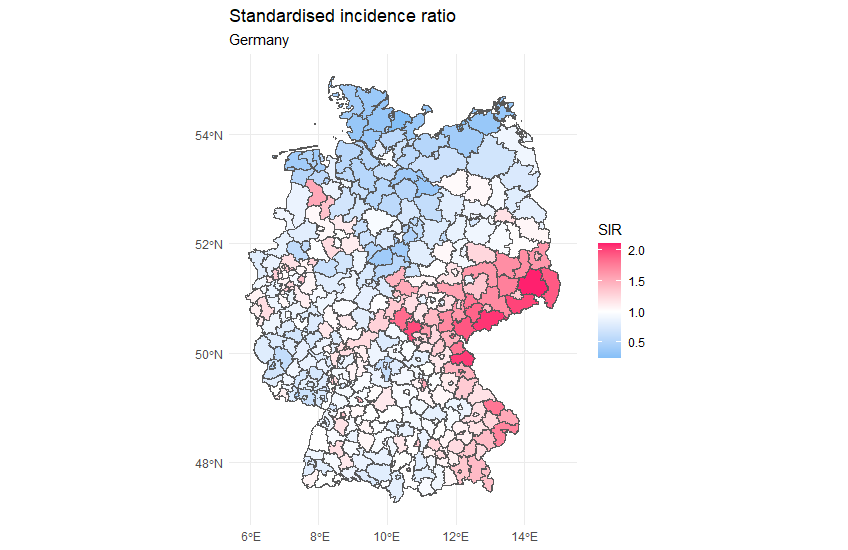
\includegraphics[width = 1.2\textwidth]{sir_germany.png}
  \caption{The standardised incidence ratio for Germany based on the data of the 24th of March 2021}
  \label{sirgermany}
\end{figure}
\subsection{Standardised Incidence Ratio for Norway}
Looking at the standardised incidence rate for Norway, a standardised incidence rate of less than 1 can be seen for most municipalities north of Trondheim. In the southern parts of Norway there are several municipalities with a rate above 1, for example the standardised incidence rate around the capital Oslo is around 2. However, the two small municipalities, Hyllestad and Ulvik, have the highest standardised incidence rate in Norway. In Hyllestad, 95 of 1328 people have been infected with Covid-19 so far, while in Ulvik, 134 of 1080 people have been infected so far. \\
The SIR in Hyllestad is around 4.5, following an outbreak in a shipyard in autumn 2020 \cite{newspaper1}, while Ulvik has a ratio of around 8, following an outbreak of the UK variant of Covid-19. According to the head of the municipality, Hans Petter Thorbjørnsen, the infections are thought to have spread through children \cite{newspaper2}. See Figure~\ref{sirnorway} for more information.
% \begin{figure}[H]
%   \centering
%   \includesvg[width = 1.2\textwidth]{sir_norway.svg}
%   \caption{The standardised incidence ratio for Norway based on the data of the 24th of March 2021}
%   \label{sirnorway}
% \end{figure}
\begin{figure}[H]
  \centering
  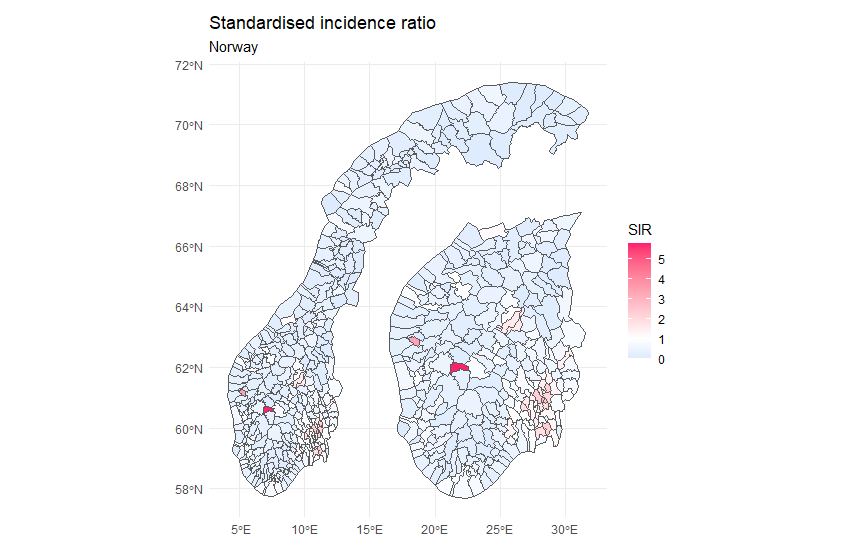
\includegraphics[width = 1.2\textwidth]{sir_norway.png}
  \caption{The standardised incidence ratio for Norway based on the data of the 24th of March 2021}
  \label{sirnorway}
\end{figure}
Because the high numbers from two small municipalities complicate the interpretation of Figure~\ref{sirnorway}, Figure~\ref{sirnorwaylog} shows the SIR on a log10 scale. It is now clearer that the standardized incidence ratio is below 1 in most parts of Norway, but that there is a higher risk in the region around Oslo.
% \begin{figure}[H]
%   \centering
%   \includesvg[width = 1.2\textwidth]{sir_norway_log.svg}
%   \caption{The log10 standardised incidence ratio for Norway based on the data of the 24th of March 2021}
%   \label{sirnorway}
% \end{figure}
\begin{figure}[H]
  \centering
  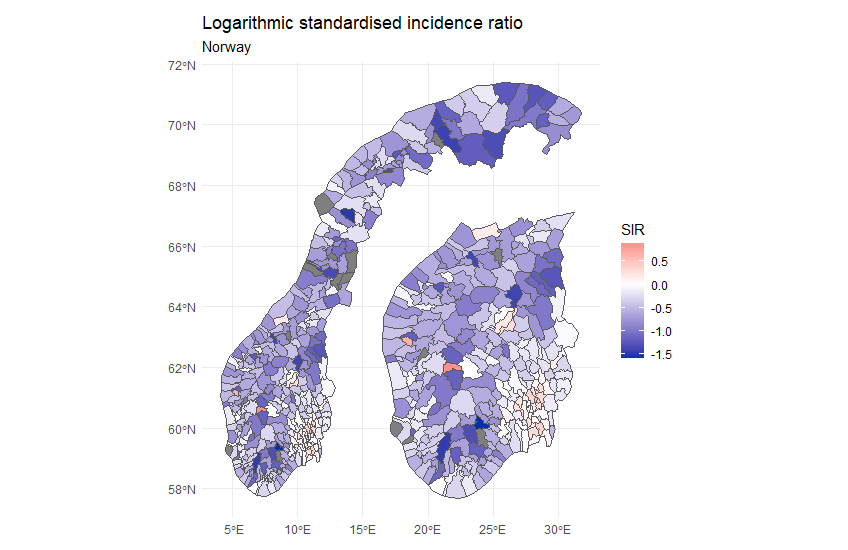
\includegraphics[width = 1.2\textwidth]{sir_norway_log.png}
  \caption{The log10 standardised incidence ratio for Norway based on the data of the 24th of March 2021}
  \label{sirnorwaylog}
\end{figure}
\clearpage
\section{Data Modelling}
After looking at the standardised incidence rates for the countries of interest, the next step is to take a closer look at the current figures for the respective countries. Spatial models are used to try to extract the factors that cause some populations to be at higher risk than other populations. Four different types of models are used for each country:
\begin{itemize}
    \item[1.] The Besarg-Yollie-Mollie Model
    \item[2.] Besags Proper Spatial Model
    \item[3.] The Leroux-Model
    \item[4.] A model without a spatial component
\end{itemize}
All of these models were computed using the INLA \cite{rinla} R package. \\
To specify each type of model, the code shown in Listing~\ref{codeModels} can be used. \\
Four measures are used to compare the models, the DIC, the WAIC, the CPO and the mean absolute error (MAE).\\
For all countries, the models were computed with
\begin{itemize}
    \item[1.] only the demographic variables as covariates
    \item[2.] only the infrastructural variables as covariates
    \item[3.] both, demographic and infrastructural variables, as covariates
\end{itemize}
In addition to specifying what type of spatial model to use, if any, there is also the option of specifying a prior. In this case, a penalised complexity prior is used for the precision $\tau$. For $\tau$, the penalised complexity prior is defined by the parameter $\sigma_0$. The equation~\ref{eq:pcprior} therefore looks like this,
\begin{equation}\label{pcprec}
    \mathbb{P}\left(\sigma > \sigma_0\right)=\alpha.
\end{equation}
The actual expression of the prior is given by
\begin{equation}
    \pi\left(\tau\right)=\frac{\lambda}{2}\tau^{-3/2}\exp\left(-\lambda\tau^{-1/2}\right),\hspace{10pt}\tau>0.
\end{equation}
Here, $\lambda=\frac{-\log\left(\alpha\right)}{\sigma_0}$ \cite{martins2014penalising}.
For the parameters $\sigma_0$ and $\alpha$, the values 1 and 0.01 were chosen. \\
The models were compared using the mean absolute error. For this, 20\% of the observations were removed from the training and used for testing instead. The predicted number of infections for these municipalities was then compared to the actual numbers.
\\
% Finally, due to the amount of covariates, forwards and backwards stepwise variable selection was performed with the intention of obtaining a model that fits the data well and at the same time is relatively easy to interpret. This can be done with the R package \texttt{INLAutils} \cite{inlautils}, as shown in Listing~\ref{codeSelection}. Backwards as well forwards variable selection was performed.\\
A list of all calculated models along with their performance measures is provided in the appendix.
\subsection{Model Selection}
Before the models are computed, however, the distribution that fits the number of cases must first be found. For this, the function \texttt{descdist()} from the \texttt{fitdistrplus} R package is used. The Cullen and Frey graph can be used to give an initial idea of which distributions fit the data, in this case the number of infections, reasonably well depending on the kurtosis and the square of the skewness. \\
The plots for Germany and Norway can be seen in Figure~\ref{cf_germany} and Figure~\ref{cf_norge}.
% \begin{figure}[H]
%     \centering
%     \includesvg[width = 0.8\textwidth]{cf_germany.svg}
%     \caption{The Cullen and Frey graph for Germany}
%     \label{cf_germany}
% \end{figure}
\begin{figure}[H]
    \centering
    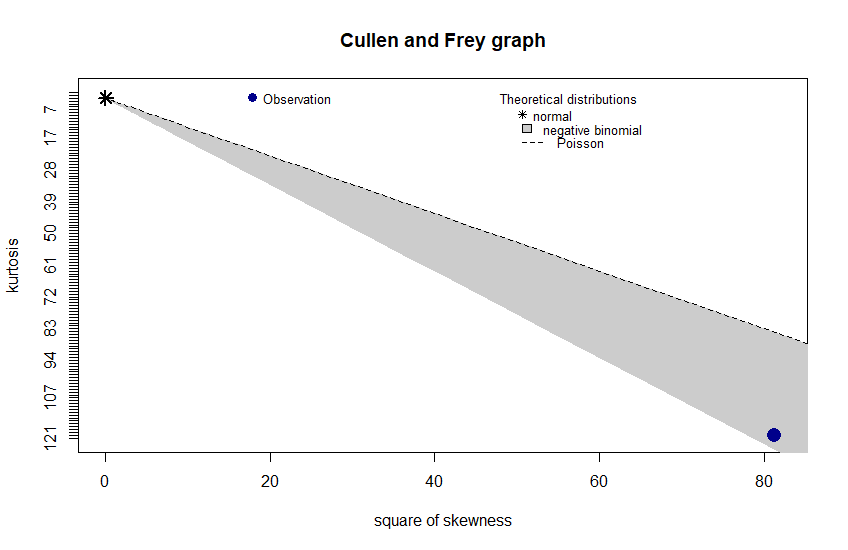
\includegraphics[width = 0.8\textwidth]{cf_germany.png}
    \caption{The Cullen and Frey graph for Germany}
    \label{cf_germany}
\end{figure}
% \begin{figure}[H]
%     \centering
%     \includesvg[width = 0.8\textwidth]{cf_norge.svg}
%     \caption{The Cullen and Frey graph for Norway}
%     \label{cf_norge}
% \end{figure}
\begin{figure}[H]
    \centering
    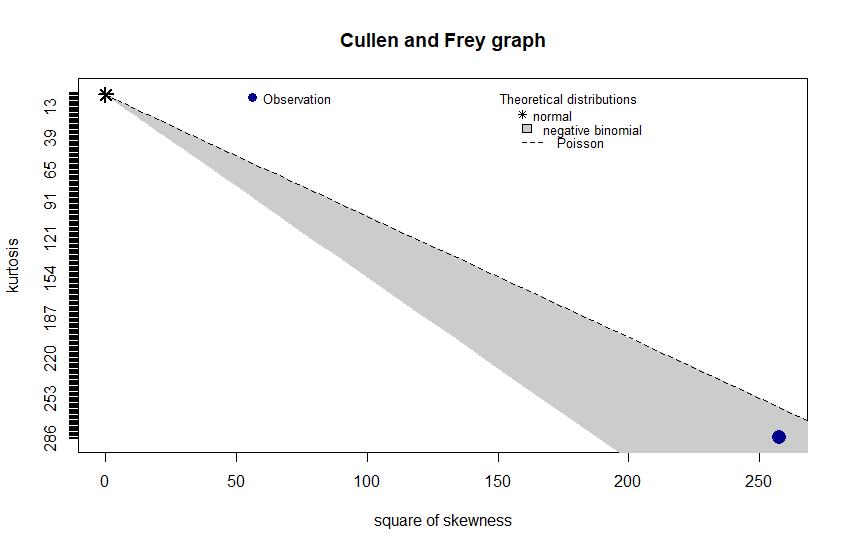
\includegraphics[width = 0.8\textwidth]{cf_norge.png}
    \caption{The Cullen and Frey graph for Norway}
    \label{cf_norge}
\end{figure}
Next, a negative binomial distribution, a normal distribution, and a Poisson distribution are fitted to the data using the maximum likelihood method. The negative binomial fits for both countries can be seen in Figure~\ref{fitNegbinomGermany} and Figure~\ref{fitNegbinomNorway}. The fits for the normal and Poisson distribution for both countries, are shown in the Appendix in Figure~\ref{fitNormalGermany}, Figure~\ref{fitPoissonGermany}, Figure~\ref{fitNormalNorway} and Figure~\ref{fitPoissonNorway}. \\
The QQ-plot for Germany and Norway looks quite similar, as there appears to be a linear relationship between the theoretical quantile and the sample quantiles, up to a certain point where the sample quantiles have a higher value than the theoretical quantiles, indicating that the distribution is right skewed. Since there are many municipalities with relatively few cases and few municipalities with a large number of cases, this is to be expected.
% \begin{figure}[H]
%     \centering
%     \includesvg[width = 0.8\textwidth]{fit_nbinom_germany.svg}
%     \caption{A negative binomial fit to the number of cases in German municipalities}
%     \label{fitNegbinomGermany}
% \end{figure}
\begin{figure}[H]
    \centering
    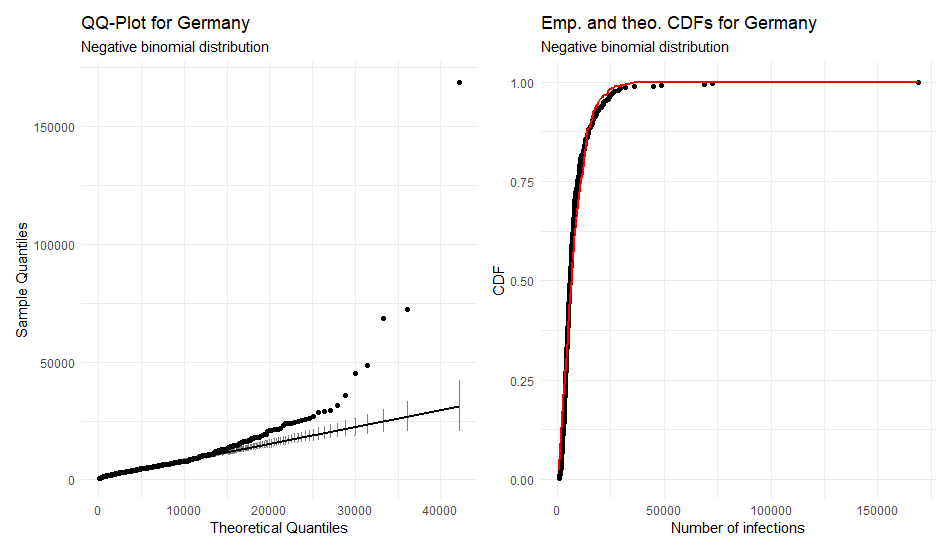
\includegraphics[width = 0.8\textwidth]{fit_nbinom_germany.png}
    \caption{A negative binomial fit to the number of cases in German municipalities}
    \label{fitNegbinomGermany}
\end{figure}
% \begin{figure}[H]
%     \centering
%     \includesvg[width = 0.8\textwidth]{fit_nbinom_norway.svg}
%     \caption{A negative binomial fit to the number of cases in Norwegian municipalities}
%     \label{fitNegbinomNorway}
% \end{figure}
\begin{figure}[H]
    \centering
    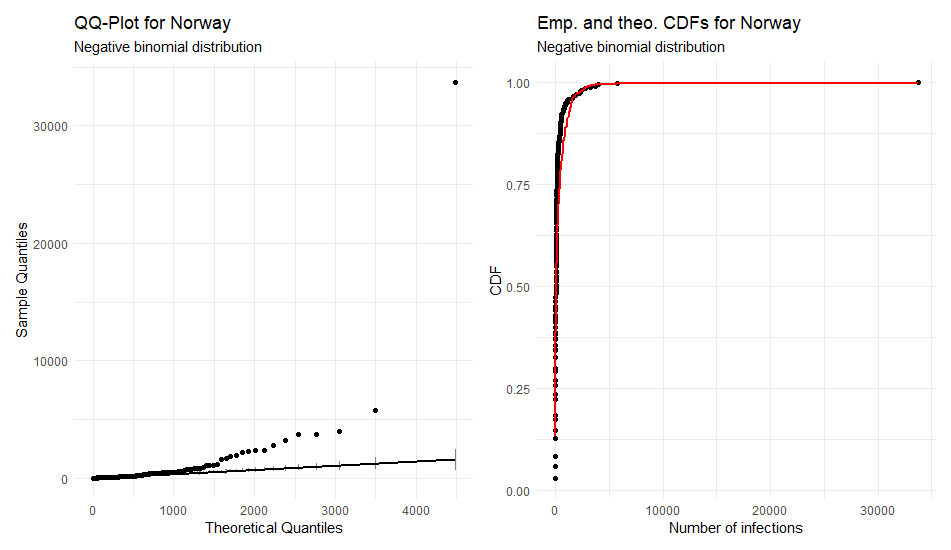
\includegraphics[width = 0.8\textwidth]{fit_nbinom_norway.png}
    \caption{A negative binomial fit to the number of cases in Norwegian municipalities}
    \label{fitNegbinomNorway}
\end{figure}
Lastly, the AIC was calculated for fitting a normal distribution to the data, a Poisson distribution to the data and a negative binomial distribution to the data. The values can be seen in Table~\ref{aic}. Afterwards, the negative binomial distribution was chosen as the distribution of the target variable in both cases. \\
\begin{table}[H] 
\caption{The AIC for different distributions for Germany and Norway \label{aic}}
\begin{tabular}{l l r}
\toprule
\textbf{Country}	& \textbf{Distribution}	& \textbf{AIC} \\
\midrule
Germany & Normal & 8360 \\
Germany & Poisson & 2148100 \\
Germany & Negative Binomial & 7731 \\
Norway & Normal & 6166 \\
Norway & Poisson & 366181 \\
Norway & Negative Binomial & 4086 \\
\bottomrule
\end{tabular}
\end{table} 
The poor fit for the Poisson distribution can be explained by looking at the range of the number of confirmed cases in a given municipality. For Germany, this number ranges from 508 to 137634 (as of March 18, 2021), while for Norway, the number ranges from 0 to 24905 (as of March 20, 2021). This results in a mean and standard deviation for Germany of 6617 and 9014, respectively. For Norway, the values for these metrics are 236 and 1389.
\clearpage
\section{Models without a Spatial Component}
To establish a baseline, we first look at models that do not include a spatial variable. To see how the values and significance of different variables change when a spatial effect is added, the models in this chapter are calculated using the same model formula that was used for the respective best performing BYM2 models in chapter~\ref{ch:spatial}. Further discussion of this is provided in the latter parts of this work. \\
For the calculated models, both the posterior mean and the credibility intervals of the coefficients were calculated to allow a better interpretation of the results. \\
To compute the posterior mean of the coefficients, the code shown in Listing~\ref{codePosteriorMean} can be used. \\
To get the expected value given a marginal function $\pi\left(x\right)$, the expected value of a function $f\left(x\right)$ is calculated, i.e.
\begin{equation*}
    \int f\left(x\right)\pi\left(x\right)dx.
\end{equation*}
To obtain a credibility interval of the fixed effects on the transformed scale, the code in Listing~\ref{codeCredibility} can be used. \\
\subsection{Models without a Spatial Component for Germany}
\subsubsection{Demographic Models}
\begin{table}[H] 
\caption{The performance measures for the demographic model. \label{demoGermany_nospatial}}
\begin{tabular}{r r r r}
\toprule\textbf{DIC}	& \textbf{WAIC} & \textbf{CPO} & \textbf{MAE}\\
\midrule
5508 & 5509 & -2754 & 174892 \\
\bottomrule
\end{tabular}
\end{table} 
\begin{table}[H]
\caption{The fixed effects for the model. Values are rounded. A $^*$ denotes a significant effect. \label{fixedDemoGermany_nospatial}}
\begin{tabular}{l r r r r c}
\toprule
\textbf{Variable}	& \textbf{Mean}	& \textbf{exp(mean$_{\hbox{p}}$)} & \textbf{exp(q0025$_{\hbox{p}}$)} & \textbf{exp(q0975$_{\hbox{p}}$)} & \textbf{sig.}\\
\midrule
(Intercept) & -0.04595 & 0.9552 & 0.9285 & 0.9826 & $^*$\\
pop\_dens & 0.1662 & 1.181& 1.134 & 1.231 &$^*$\\
FDP & 0.05825 & 1.060& 1.024 & 1.097 &$^*$\\
urb\_dens & 0.01592 & 1.016 & 0.9773& 1.057 &\\
die\_linke & -0.05957 & 0.9423 & 0.9108 & 0.9748 & $^*$\\
SPD & -0.1362 & 0.8728 & 0.8453 & 0.9010 & $^*$\\
Gruene & -0.2391 & 0.7875 & 0.7553 & 0.8208 & $^*$\\
\bottomrule
\end{tabular}
\end{table}
\subsubsection{Infrastructure Models}
\begin{table}[H] 
\caption{The performance measures for the infrastructure model. \label{infraGermany_nospatial}}
\begin{tabular}{r r r r}
\toprule\textbf{DIC}	& \textbf{WAIC} & \textbf{CPO} & \textbf{MAE}\\
\midrule
5679 & 5680 & -2862 & 175480 \\
\bottomrule
\end{tabular}
\end{table}
\begin{table}[H]
\caption{The fixed effects for the model. Values are rounded. A $^*$ denotes a significant effect. \label{FixedInfraGermany_nospatial}}
\begin{tabular}{l r r r r c}
\toprule
\textbf{Variable}	& \textbf{Mean}	& \textbf{exp(mean$_{\hbox{p}}$)} & \textbf{exp(q0025$_{\hbox{p}}$)} & \textbf{exp(q0975$_{\hbox{p}}$)} & \textbf{sig.}\\
\midrule
(Intercept) & -0.03036 & 0.9703 & 0.9355 & 1.006 & \\
pop\_dens & 0.09421 & 1.099 & 1.037 & 1.165 & $^*$\\
place\_of\_worship & 0.03847 & 1.040 & 0.9916 & 1.089\\
clinic & 0.03075 & 1.032 & 0.9593 & 1.111  \\
nursing\_home & 0.02336 & 1.024 & 0.9795 & 1.071 \\
aerodrome & -0.01383 & 0.9864 & 0.9574 & 1.020 \\
platform & -0.01583 & 0.9848 & 0.9235 & 1.050 \\
higher\_education & -0.03884 & 0.9623 & 0.9140 & 1.015 \\
retail & -0.04742 & 0.9542 & 0.8949 & 1.018 \\
urb\_dens & -0.05078 & 0.9508 & 0.9050 & 0.9995 & $^*$\\
\bottomrule
\end{tabular}
\end{table}
\subsubsection{Models with Demographic and Infrastructure Variables}
\begin{table}[H] 
\caption{The performance measures for the demographic + infrastructure model. \label{allGermany_nospatial}}
\begin{tabular}{r r r r}
\toprule
\textbf{DIC}	& \textbf{WAIC} & \textbf{CPO} & \textbf{MAE}\\
\midrule
5509 & 5509 & -2765 &  176320 \\
\bottomrule
\end{tabular}
\end{table}
\begin{table}[H]
\caption{The fixed effects for the model. Values are rounded. A $^*$ denotes a significant effect. \label{FixedAllGermany_nospatial}}
\begin{tabular}{l r r r r c}
\toprule
\textbf{Variable}	& \textbf{Mean}	& \textbf{exp(mean$_{\hbox{p}}$)} & \textbf{exp(q0025$_{\hbox{p}}$)} & \textbf{exp(q0975$_{\hbox{p}}$)} & \textbf{sig.}\\
\midrule
(Intercept) & -0.06241 & 0.9396 & 0.9119 & 0.9681 & $^*$\\
pop\_dens & 0.1619 & 1.176 & 1.123 & 1.232 & $^*$\\
FDP & 0.04973 & 1.051 & 1.013 & 1.090 & $^*$\\
sex & 0.03509 & 1.036 & 1.001 & 1.072 & $^*$\\
platform & 0.02336 & 1.024 & 0.9712 & 1.079 \\
urb\_dens & 0.01444 & 1.015 & 0.9736 & 1.058 \\
nursing\_home & 0.01117 & 1.011 & 0.9775 & 1.047 \\
higher\_education & 0.009667 & 1.010 & 0.9693 & 1.053 \\
clinic & 0.003535 & 1.004 & 0.9506 & 1.061 \\
aerodrome & -0.0006104 & 0.9995 & 0.9730 & 1.029 \\
retail & -0.009684 & 0.9907 & 0.9427 & 1.041 \\
place\_of\_worship & -0.02004 & 0.9804 & 0.9402 & 1.022 \\
log(trade\_tax) & -0.05178 & 0.9497 & 0.9184 & 0.9811 & $^*$\\
die\_linke & -0.08194 & 0.9215 & 0.8858 & 0.9584 & $^*$\\
SPD & -0.1447 & 0.8654 & 0.8369 & 0.8947 & $^*$\\
Gruene & -0.2698 & 0.7638 & 0.7285 & 0.8003 & $^*$\\
\bottomrule
\end{tabular}
\end{table}
\subsection{Models without a Spatial Component for Norway}
\subsubsection{Demographic Models}
\begin{table}[H] 
\caption{The performance measures for the demographic model. \label{demoNorway_nospatial}}
\begin{tabular}{r r r r}
\toprule\textbf{DIC}	& \textbf{WAIC} & \textbf{CPO} & \textbf{MAE}\\
\midrule
2785 & 2792 & -1491 & 8210 \\
\bottomrule
\end{tabular}
\end{table} 
\begin{table}[H]
\caption{The fixed effects for the model. Values are rounded. A $^*$ denotes a significant effect. \label{fixedDemoNorway_nospatial}}
\begin{tabular}{l r r r r c}
\toprule
\textbf{Variable}	& \textbf{Mean}	& \textbf{exp(mean$_{\hbox{p}}$)} & \textbf{exp(q0025$_{\hbox{p}}$)} & \textbf{exp(q0975$_{\hbox{p}}$)} & \textbf{sig.}\\
\midrule
(Intercept) & -0.7715 & 0.4629 & 0.4189 & 0.5114 & $^*$ \\
urb\_dens & 0.3323 & 1.399 & 1.192 & 1.674 & $^*$ \\
sex & -0.09652 & 0.9095 & 0.8132 & 1.015 \\
\bottomrule
\end{tabular}
\end{table}
\subsubsection{Infrastructure Models}
\begin{table}[H] 
\caption{The performance measures for the infrastructure model. \label{infraNorway_nospatial}}
\begin{tabular}{r r r r}
\toprule\textbf{DIC}	& \textbf{WAIC} & \textbf{CPO} & \textbf{MAE}\\
\midrule
2786 & 2793 & -1670 & 13022 \\
\bottomrule
\end{tabular}
\end{table} 
\begin{table}[H]
\caption{The fixed effects for the model. Values are rounded. A $^*$ denotes a significant effect. \label{fixedInfraNorway_nospatial}}
\begin{tabular}{l r r r r c}
\toprule
\textbf{Variable}	& \textbf{Mean}	& \textbf{exp(mean$_{\hbox{p}}$)} & \textbf{exp(q0025$_{\hbox{p}}$)} & \textbf{exp(q0975$_{\hbox{p}}$)} & \textbf{sig.}\\
\midrule
(Intercept) & -0.7764 & 0.4607 & 0.4170 & 0.5088 & $^*$ \\
urb\_dens & 0.3824 & 1.474 & 1.207 & 1.823 & $^*$ \\
platform & 0.1625 & 1.183 & 0.9634 & 1.469 \\
nursing\_home & 0.03350 & 1.035 & 0.9461 & 1.154\\
place\_of\_worship & 0.01994 &1.024 & 0.8687 & 1.213 \\
marketplace & 0.01059 & 1.014 & 0.8782 & 1.183 \\
higher\_education & 0.004825 & 1.006 & 0.9139 & 1.126 \\
aerodrome & -0.1419 & 0.8699 & 0.7437 & 0.9848 & $^*$ \\
office & -0.2362 & 0.7930 & 0.6642 & 0.9530 & $^*$ \\
\bottomrule
\end{tabular}
\end{table}
\subsubsection{Models with Demographic and Infrastructure Variables}
\begin{table}[H] 
\caption{The performance measures for the demographic + infrastructure model. \label{allNorway_nospatial}}
\begin{tabular}{r r r r}
\toprule\textbf{DIC}	& \textbf{WAIC} & \textbf{CPO} & \textbf{MAE}\\
\midrule
2713 & 2718 & -1623 & 10170 \\
\bottomrule
\end{tabular}
\end{table} 
\begin{table}[H]
\caption{The fixed effects for the model. Values are rounded. A $^*$ denotes a significant effect. \label{fixedAllNorway_nospatial}}
\begin{tabular}{l r r r r c}
\toprule
\textbf{Variable}	& \textbf{Mean}	& \textbf{exp(mean$_{\hbox{p}}$)} & \textbf{exp(q0025$_{\hbox{p}}$)} & \textbf{exp(q0975$_{\hbox{p}}$)} & \textbf{sig.}\\
\midrule
(Intercept) & -0.8721 & 0.4185 & 0.3832 & 0.4569 & $^*$ \\
immigrants\_ & \multirow{2}{*}{0.2773}& \multirow{2}{*}{1.322}& \multirow{2}{*}{1.165}& \multirow{2}{*}{1.497}& \multirow{2}{*}{$^*$}\\
\_total \\
unemp\_immg & 0.2086 & 1.236 & 1.062 & 1.435 & $^*$ \\
urb\_dens & 0.1790 & 1.200 & 1.027 & 1.423 & $^*$ \\
unemp\_tot & 0.07675 & 1.085 & 0.8969 & 1.304 \\
platform & 0.07141 & 1.078 & 0.9139 & 1.271 \\
higher\_ & \multirow{2}{*}{0.01850}& \multirow{2}{*}{1.020}& \multirow{2}{*}{0.9375}& \multirow{2}{*}{1.125}\\ 
education \\
nursing\_home & 0.01501 & 1.016 & 0.9377 & 1.117 \\
median\_age & -0.004360  & 0.9969 & 0.9020 & 1.098 \\
marketplace & -0.006536 & 0.9959 & 0.8735 & 1.145 \\
place\_of\_ & \multirow{2}{*}{-0.04057}& \multirow{2}{*}{0.9634}& \multirow{2}{*}{0.8233}& \multirow{2}{*}{1.130} \\
worship \\
office & -0.1372 & 0.8749 & 0.7434 & 1.030 \\
sex & -0.1535 & 0.8591 & 0.7691 & 0.9568 & $^*$ \\
aerodrome & -0.1954 & 0.8247 & 0.7010 & 0.9335 & $^*$ \\
\bottomrule
\end{tabular}
\end{table}
\clearpage
\section{Spatial Models}\label{ch:spatial}
\subsection{Spatial Models for Germany}
First, a look is taken at the spatial models calculated for Germany. These models are based on data from 24 March 2021, when 2.695.037 people in Germany were confirmed infected with Covid-19. The five municipalities with the most infections are shown in Table~\ref{top5germany}.
\begin{table}[H] 
\caption{The municipalities with the most infections as of March 24th 2021. \label{top5germany}}
\begin{tabular}{l r r}
\toprule
\textbf{Municipality}	& \textbf{Population}	& \textbf{Number of infections} \\
\midrule
SK Berlin & 3644826 & 141639   \\     
SK Hamburg & 1841179 & 58661   \\
SK Munich & 1471508 & 57690   \\
SK Cologne & 1085664 & 37592   \\
Region Hannover & 1157624 & 36241   \\
\bottomrule
\end{tabular}
\end{table}
\subsubsection{Demographic Models}\label{sssec:demoGermany}
The model with the best performance based on the demographic variables was a Leroux model computed using the formula in Listing~\ref{codeDemoGermany}. The variables used for this model were the percentages of the vote for the six biggest German political parties. \\
The performance measures of this model and the best-performing BYM2 and Besag proper models are shown in Table~\ref{demoGermany}. 
\begin{table}[H] 
\caption{The performance measures for the best performing demographic model of each type. \label{demoGermany}}
\begin{tabular}{l r r r r}
\toprule
\textbf{Model}	& \textbf{DIC}	& \textbf{WAIC} & \textbf{CPO} & \textbf{MAE}\\
\midrule
Besag  & 4706 & 4749 & -2756 &  176861 \\
BYM2 & 4624 & 4593  & -2702 &  176747\\
Leroux & 4807  & 4830 & -3237 & 175780\\
\bottomrule
\end{tabular}
\end{table}
The summary of the fixed effects is shown in Table~\ref{fixedDemoGermany_spatial}.
\begin{table}[H]
\caption{The fixed effects for the model. Values are rounded. A $^*$ denotes a significant effect. \label{fixedDemoGermany_spatial}}
\begin{tabular}{l r r r r c}
\toprule
\textbf{Variable}	& \textbf{Mean}	& \textbf{exp(mean$_{\hbox{p}}$)} & \textbf{exp(q0025$_{\hbox{p}}$)} & \textbf{exp(q0975$_{\hbox{p}}$)} & \textbf{sig.}\\
\midrule
(Intercept) & -0.07886 & 0.9242 & 0.9124 & 0.9362 & $^*$\\
pop\_dens & 0.1061 & 1.112 & 1.076 & 1.149 &$^*$\\
FDP & 0.02740 & 1.028 & 0.9873 & 1.070 &\\
urb\_dens & 0.01133 & 1.012 & 0.9823 & 1.041 &\\
die\_linke & 0.002600 & 1.003 & 0.9540 & 1.054 & \\
SPD & -0.03264 & 0.9681 & 0.9253 & 1.012 &\\
Gruene & -0.1654 & 0.8478 & 0.8119 & 0.8848 & $^*$\\
\bottomrule
\end{tabular}
\end{table}
% Wondreys and Mudde took a look at right-wing parties' responses to the pandemic, pointing out that while these parties were quick to warn about the virus, once cases spiked they criticised the measures taken to contain the spread of the virus. They also noted that right-wing parties supported demonstrations against these measures. However, they also stressed that these parties often rejected the measures proposed by the leading parties because they themselves were part of the opposition, as is the case with the AfD in Germany \cite{wondreys2020victims}.  \\
% Farias and Pilati also conducted a study in Brazil to predict social distancing violation intention and past non-compliance during the COVID-19 pandemic, controlling for the effects of intolerance of uncertainty and sociodemographic variables. Their results included that individuals who support right-wing parties are more likely to violate social distancing measures \cite{farias2020violating}. \\
% An increase by one standard deviation for the AfD leads to a risk increase of about 16.7\%. No significant effects were observed for all other parties. \\
\subsubsection{Infrastructure Models}\label{sssec:infraGermany}
When it comes to the models based on the infrastructural variables, a BYM2 model performed the best. It was computed using formula in Listing~\ref{codeInfraGermany}. \\
The performance measures of this model and the best-performing other models are shown in Table~\ref{infraGermany}
\begin{table}[H] 
\caption{The performance measures for the best performing infrastructure model of each type. \label{infraGermany}}
\begin{tabular}{l r r r r}
\toprule
\textbf{Model}	& \textbf{DIC}	& \textbf{WAIC} & \textbf{CPO} & \textbf{MAE}\\
\midrule
Besag & 4688 & 4673 & -2762 & 176473\\
BYM2 & 4633 & 4619 & -2760 & 176197\\
Leroux & 4749 & 4772 & -3093 & 177001\\
\bottomrule
\end{tabular}
\end{table}
The values of the covariates are shown in Table~\ref{FixedInfraGermany_spatial}.
\begin{table}[H]
\caption{The fixed effects for the model. Values are rounded. A $^*$ denotes a significant effect. \label{FixedInfraGermany_spatial}}
\begin{tabular}{l r r r r c}
\toprule
\textbf{Variable}	& \textbf{Mean}	& \textbf{exp(mean$_{\hbox{p}}$)} & \textbf{exp(q0025$_{\hbox{p}}$)} & \textbf{exp(q0975$_{\hbox{p}}$)} & \textbf{sig.}\\
\midrule
(Intercept) & -0.07993 & 0.9232 & 0.9108 & 0.9358 & $^*$\\
pop\_dens & 0.08988 & 1.094 & 1.049 & 1.140 & $^*$\\
retail & 0.04115 & 1.042 & 1.002 & 1.084 & $^*$\\
place\_of\_ & \multirow{2}{*}{0.02528} & \multirow{2}{*}{1.026} & \multirow{2}{*}{0.9916} & \multirow{2}{*}{1.061}\\
worship\\
nursing\_ & \multirow{2}{*}{0.01689} & \multirow{2}{*}{1.017} & \multirow{2}{*}{0.9907} & \multirow{2}{*}{1.044} \\
home\\
aerodrome & 0.007450 & 1.008 & 0.9893 & 1.026 \\
platform & -0.01111 & 0.9892 & 0.9473 & 1.032 \\
urb\_dens & -0.01248 & 0.9877 & 0.9544 & 1.022 \\
clinic & -0.02707 & 0.9735 & 0.9319 & 1.016  \\
higher\_ & \multirow{2}{*}{-0.05918} & \multirow{2}{*}{0.9427} & \multirow{2}{*}{0.9076} & \multirow{2}{*}{0.9788} & \multirow{2}{*}{$^*$} \\
education\\
\bottomrule
\end{tabular}
\end{table}
% Findings from these results are that bakeries, places of worship and population density increase the risk of infection. For bakeries, an increase of 1 standard deviation leads to a risk increase of 68.3\%. Bakeries are relatively widespread in Germany and many people go there several times a week to get fresh bread or other baked goods. When many people congregate in bakeries, viruses can spread more easily. \\
% A 1 standard deviation increase in population density leads to an 11.6\% increase in relative risk, which should not be too surprising since in communities with higher population density, people come into contact with more people, which in turn helps the virus move from host to host. \\
% Finally, places of worship were not closed for a long time in Germany due to freedom of religion and therefore people gathered in churches, mosques and the like. A 1 standard deviation increase in these places of worship therefore leads to a 9.5\% increase in the risk of contracting Covid-19. \\
% Yezli and Khan's paper argues for the closure of these places of worshipon the grounds that they pose a risk of transmitting COVID-19 to potentially large numbers of people through a single case. Gatherings at these places often involve dense mixing of many people in a confined space, sometimes for long periods of time \cite{yezli2020covid}.
\subsubsection{Demographic + Infrastructure Models}
Finally, models are considered that include both the infrastructural and demographic covariates. \\
The best performing model was again a BYM2 model, computed with the formula shown in Listing~\ref{codeBothGermany}. \\
The performance measures of the computed models are shown in Table~\ref{allGermany}.
\begin{table}[H] 
\caption{The performance measures for the best performing demographic + infrastructure model of each type. \label{allGermany}}
\begin{tabular}{l r r r r}
\toprule
\textbf{Model}	& \textbf{DIC}	& \textbf{WAIC} & \textbf{CPO} & \textbf{MAE}\\
\midrule
Besag&  4734 & 4776 & -2769 & 174662\\
BYM2 & 4645 & 4617 & -2729 & 174514\\
Leroux & 5281 & 5296 & -2939 & 176316 \\
\bottomrule
\end{tabular}
\end{table}
The fixed effects are shown in Table~\ref{FixedAllGermany_spatial}.
\begin{table}[H]
\caption{The fixed effects for the model. Values are rounded. A $^*$ denotes a significant effect. \label{FixedAllGermany_spatial}}
\begin{tabular}{l r r r r c}
\toprule
\textbf{Variable}	& \textbf{Mean}	& \textbf{exp(mean$_{\hbox{p}}$)} & \textbf{exp(q0025$_{\hbox{p}}$)} & \textbf{exp(q0975$_{\hbox{p}}$)} & \textbf{sig.}\\
\midrule
(Intercept) & -0.08509 & 0.9185 & 0.9043 & 0.9328 & $^*$\\
pop\_dens & 0.1119 & 1.119 & 1.073 & 1.166 & $^*$\\
retail & 0.02242 & 1.023 & 0.9844 & 1.062 \\
nursing\_ & \multirow{2}{*}{0.01572} & \multirow{2}{*}{1.016} & \multirow{2}{*}{0.9908} & \multirow{2}{*}{1.042} \\
home \\
FDP & 0.01296 & 1.013 & 0.9703 & 1.058 &\\
die\_linke & 0.008281 & 1.009 & 0.9568 & 1.063\\
aerodrome & 0.007271 & 1.007 & 0.9892 & 1.026 \\
platform & 0.006828 & 1.007 & 0.9662 & 1.049 \\
urb\_dens & 0.006776 & 1.007 & 0.9740 & 1.041 \\
sex & 0.001694 & 1.002 & 0.9716 & 1.033 &\\
place\_of\_ & \multirow{2}{*}{-0.001927} & \multirow{2}{*}{0.9982} & \multirow{2}{*}{0.9646} & \multirow{2}{*}{1.033} \\
worship \\
clinic & -0.003287 & 0.9969 & 0.9559 & 1.039 \\
log & \multirow{2}{*}{-0.01374} & \multirow{2}{*}{0.9864} & \multirow{2}{*}{0.9617} & \multirow{2}{*}{1.011}\\
trade\_tax \\
SPD & -0.03573 & 0.9652 & 0.9204 & 1.012 \\
higher\_ & \multirow{2}{*}{-0.03595} & \multirow{2}{*}{0.9649} & \multirow{2}{*}{0.9297} & \multirow{2}{*}{1.001} \\
education \\
Gruene & -0.1570 & 0.8550 & 0.8122 & 0.8994 & $^*$\\
\bottomrule
\end{tabular}
\end{table}
According to this model, the three biggest driving factors for the number of infections are the amount of unemployed foreigners, the share of the vote for the AfD and the population density. The influence of the AfD was already discussed in Section~\ref{sssec:demoGermany}, only in this case an increase of 1 standard deviation leads to a risk increase of 22.5\%. In Section~\ref{sssec:infraGermany} population density was discussed. Here, a 1 standard deviation increase leads to a 13.3\% increase in relative risk. For unemployed foreigners, a 1 standard deviation increase leads to a 95.4\% increase in risk. \\
Other factors that positively influence the risk of infection are the number of schools, the proportion of women in the population and the number of higher educational institutions. A 1 standard deviation increase in the number of schools leads to a 12.7\% increase in risk, which could be an indicator that schools should remain closed because so many children from different households meet there, providing a good place for a virus to spread. Schools in Germany actually closed relatively late, and did reopen at the beginning of 2021.\\
A 1 standard deviation increase in the proportion of women leads to a 6.7\% increase in risk and for higher education buildings a 1 standard deviation increase leads to a 6.5\% increase in risk. 
\subsection{Spatial Models for Norway}
Next, the same types of models are evaluated for Norway. These models are based on data from 24 March 2021, when 87537 people in Norway were confirmed infected with Covid-19. The five municipalities with the most infections are shown in Table~\ref{top5norway}.
\begin{table}[H] 
\caption{The municipalities with the most infections as of March 24th 2021. \label{top5norway}}
\begin{tabular}{l r r}
\toprule
\textbf{Municipality}	& \textbf{Population}	& \textbf{Number of infections} \\
\midrule
Oslo & 693494 & 26151 \\
Bergen & 283929 & 4738 \\
Drammen & 101386 & 3149 \\
Bærum & 127731 & 2834 \\
Lillestrøm & 85983 & 2779 \\
\bottomrule
\end{tabular}
\end{table}
\subsubsection{Demographic Models}\label{sssec:demoNorway}
The best demographic model was a Leroux model calculated using the formula shown in Listing~\ref{codeDemoNorway}. \\
The performance measures for all models are shown in Table~\ref{demoNorway}. It is noticeable that the mean error in Norway is significantly smaller, suggesting that the models for Germany have greatly overestimated or underestimated the number of infections.
\begin{table}[H] 
\caption{The performance measures for the best performing demographic model of each type. \label{demoNorway}}
\begin{tabular}{l r r r r}
\toprule
\textbf{Model}	& \textbf{DIC}	& \textbf{WAIC} & \textbf{CPO} & \textbf{MAE}\\
\midrule
Besag  & 2321 & 2340 & -8261 & 9578 \\
BYM2 & 2258 & 2225 & -7170 & 9393\\
Leroux & 2263  & 2222 & -8083 & 7797\\
\bottomrule
\end{tabular}
\end{table}
All other performance measures for these models are also lower than for the models computed for Germany. \\
The effects of the covariates are shown in Table~\ref{fixedDemoNorway_spatial}.
\begin{table}[H] 
\caption{The fixed effects for the model without a spatial component. Values are rounded. A $^*$ denotes a significant effect.\label{fixedDemoNorway_spatial}}
\begin{tabular}{l r r r r c}
\toprule
\textbf{Variable}	& \textbf{Mean}	& \textbf{exp(mean$_{\hbox{p}}$)} & \textbf{exp(q0025$_{\hbox{p}}$)} & \textbf{exp(q0975$_{\hbox{p}}$)} & \textbf{sig.}\\
\midrule
(Intercept) & -1.109 & 0.3299 & 0.3085 & 0.3519 & $^*$ \\
urb\_dens & 0.07558 & 1.079 & 1.005 & 1.157 & $^*$ \\
sex & 0.01448 & 1.016 & 0.9214 & 1.117 \\
\bottomrule
\end{tabular}
\end{table}
% The only significant influence on the number of infections is the total number of unemployed people in a municipality. A 1 standard deviation increase in total unemployment leads to a 46.6\% increase in the risk. A possible explanation for this could be that the unemployed spend less time at home and instead move around more and thus have more contact with people, but this should be taken with a grain of salt.
\subsubsection{Infrastructure Models}
For the models based on the infrastructure variables, the best predictive performance was observed for a Besag model. The formula is shown in Listing~\ref{codeInfraNorway}. \\
The performance measure for the models is shown in Table~\ref{infraNorway}.
\begin{table}[H] 
\caption{The performance measures for the best performing infrastructure model of each type. \label{infraNorway}}
\begin{tabular}{l r r r r}
\toprule
\textbf{Model}	& \textbf{DIC}	& \textbf{WAIC} & \textbf{CPO} & \textbf{MAE} \\
\midrule
Besag  & 2327 & 2334 & -8171 & 10581 \\
BYM2 & 2258 & 2224 & -6978 & 10717\\
Leroux &  2275 & 2228 & -9023 & 12244\\
\bottomrule
\end{tabular}
\end{table}
The effect of the covariates are shown in Table~\ref{fixedInfraNorway_spatial}.
\begin{table}[H]
\caption{The fixed effects for the model. Values are rounded. A $^*$ denotes a significant effect. \label{fixedInfraNorway_spatial}}
\begin{tabular}{l r r r r c}
\toprule
\textbf{Variable}	& \textbf{Mean}	& \textbf{exp(mean$_{\hbox{p}}$)} & \textbf{exp(q0025$_{\hbox{p}}$)} & \textbf{exp(q0975$_{\hbox{p}}$)} & \textbf{sig.}\\
\midrule
(Intercept) & -1.115 & 0.3282 & 0.3062 & 0.3508 & $^*$ \\
place\_of\_ & \multirow{2}{*}{0.1504} & \multirow{2}{*}{1.165} & \multirow{2}{*}{1.019} & \multirow{2}{*}{1.328} & \multirow{2}{*}{$^*$} \\
worship\\
urb\_dens & 0.05900 & 1.063 & 0.9386 & 1.201 &  \\
nursing\_ & \multirow{2}{*}{0.02292} & \multirow{2}{*}{1.024} & \multirow{2}{*}{0.9434} & \multirow{2}{*}{1.110}\\
home\\
higher\_ & \multirow{2}{*}{0.008234} & \multirow{2}{*}{1.009} & \multirow{2}{*}{0.9344} & \multirow{2}{*}{1.087} \\
education\\
marketplace & -0.003012 & 0.9989 & 0.8838 & 1.113 \\
platform & -0.01936 & 0.9838 & 0.8428 & 1.142 \\
aerodrome & -0.05807 & 0.9456 & 0.8212 & 1.059  \\
office & -0.0788 & 0.9273 & 0.7866 & 1.083  \\
\bottomrule
\end{tabular}
\end{table}
\subsubsection{Demographic + Infrastructure Models}
For the models containing variables related to the demographic of Norway and the infrastructure, again a Besag model performed the best. Its formula can be seen in Listing~\ref{codeBothNorway}. \\
The performance measures for the models are shown in Table~\ref{allNorway}
\begin{table}[H] 
\caption{The performance measures for the best performing demographic + infrastructure model of each type. \label{allNorway}}
\begin{tabular}{l r r r r}
\toprule
\textbf{Model}	& \textbf{DIC}	& \textbf{WAIC} & \textbf{CPO} & \textbf{MAE} \\
\midrule
Besag  & 2452 & 2468 & -3782 & 11266 \\
BYM2 & 2278 & 2265 & -5627 & 11520\\
Leroux &  2272 & 2230 & -8261 & 11434\\
\bottomrule
\end{tabular}
\end{table}
The fixed effects are shown in Table~\ref{fixedAllNorway_spatial}.
\begin{table}[H]
\caption{The fixed effects for the model. Values are rounded. A $^*$ denotes a significant effect. \label{fixedAllNorway_spatial}}
\begin{tabular}{l r r r r c}
\toprule
\textbf{Variable}	& \textbf{Mean}	& \textbf{exp(mean$_{\hbox{p}}$)} & \textbf{exp(q0025$_{\hbox{p}}$)} & \textbf{exp(q0975$_{\hbox{p}}$)} & \textbf{sig.}\\
\midrule
(Intercept) & -1.121 & 0.3260 & 0.3026 & 0.3504 & $^*$ \\
immigrants\_ & \multirow{2}{*}{0.1432} & \multirow{2}{*}{1.156} & \multirow{2}{*}{1.029} & \multirow{2}{*}{1.294} & \multirow{2}{*}{$^*$} \\
total \\
unemp\_tot & 0.08298 & 1.090 & 0.9203 & 1.281 \\
place\_of\_ & \multirow{2}{*}{0.08127} & \multirow{2}{*}{1.087} & \multirow{2}{*}{0.9488} & \multirow{2}{*}{1.242} \\
worship \\
unemp\_immg & 0.06734 & 1.073 & 0.9247 & 1.237 & \\
urb\_dens & 0.04398 & 1.047 & 0.9284 & 1.178 \\
marketplace & 0.01543 & 1.017 & 0.9041 & 1.142 \\
nursing\_ & \multirow{2}{*}{0.008396} & \multirow{2}{*}{1.009} & \multirow{2}{*}{0.9340} & \multirow{2}{*}{1.089} \\
home \\
higher\_ & \multirow{2}{*}{0.005382} & \multirow{2}{*}{1.006} & \multirow{2}{*}{0.9325} & \multirow{2}{*}{1.083} \\
education\\
sex & 0.004273 & 1.006 & 0.9073 & 1.112\\
platform & -0.02252 & 0.9805 & 0.8450 & 1.131 \\
office & -0.06488 & 0.9402 & 0.8004 & 1.095 \\
aerodrome & -0.09666 & 0.9097 & 0.7926 & 1.015 \\
median\_age & -0.1151  & 0.8925 & 0.8052 & 0.9853 & $^*$ \\
\bottomrule
\end{tabular}
\end{table}
\clearpage
\subsection{Discussion of the Spatial Models}
For the discussion of the results of this part of the analysis, a look is first taken at the differences between the models calculated without a spatial component and the models with such a component. For the latter, a more in-depth analysis of the results is also carried out.
\subsubsection{Discussion of the Models for Germany}
\paragraph{Demographic Models}\label{par:demoGermany} $\newline$
Comparing Table~\ref{demoGermany_nospatial} and Table~\ref{demoGermany}, it can be seen that the model without spatial component performs slightly better in terms of the mean absolute error, equally well in terms of the CPO and worse in terms of the DIC and WAIC. \\
In the model without the spatial component, all variables except urban density had a significant effect, whereas in the BYM2 model only the urban density and the percentage of the vote for the Greens had a significant effect. \\
The posterior mean of the intercept implies a -7.6\% risk rate across Germany with a credibility interval ranging from -8.8\% to -6.4\%. \\
An increase in the population density by 1 standard deviation leads to an increase in the relative risk of infection by 11.2\%  which should not be too surprising since in communities with higher population density, people come into contact with more people, which in turn helps the virus move from host to host. Several studies have also linked higher population density to a variety of other factors, e.g. cities with higher population density tend to have outbreaks earlier than smaller cities, and crowding can also affect the spread of the virus \autocite[][]{carozzi2020urban}. In general, however, several papers have found a correlation between higher population density and a higher risk of contracting covid-19 \autocite[][]{pequeno2020air, cocskun2021spread, kadi2020population}.
\\
A 1 standard deviation increase in the percentage of the vote for the Greens reduces the relative risk of infection by around 15.2\%. In Germany, the Greens are on the left of the political spectrum, as are the SPD and the party "Die Linke", the latter being on the far left. A 2021 study by Gadarian et. al. examined the US population's health behaviours, attitudes and political opinions on COVID-19 in the first weeks of the national health crisis. Their findings included that people who identified more with the Democrat party were more likely to follow the guidelines than people who identified with the more right-wing Republican party \autocite[][]{gadarian2021partisanship}. This supports the theory that areas where the left-leaning Greens get more votes are also areas where the risk of infection is lower.
\\
In Figure~\ref{posteriorGermanyDemo} it can be seen that the relative risk for large parts of Germany is above 1, except for most of northern Germany and some parts in the southwest of the country. The posterior probability is highest for parts of North Rhine-Westphalia, Germany's most populous conurbation, the Ruhr region, Saxony and Thuringia, and parts of Bavaria and Baden-Württemberg. The higher numbers in Bavaria can be explained by the large common borders with Austria and the Czech Republic, two countries that were more affected by the pandemic. Many people cross these borders because of tourism and many guest workers come from the Czech Republic to work on agricultural land in Bavaria, which led to several Covid 19 outbreaks.
\begin{figure}[H]
    \centering
    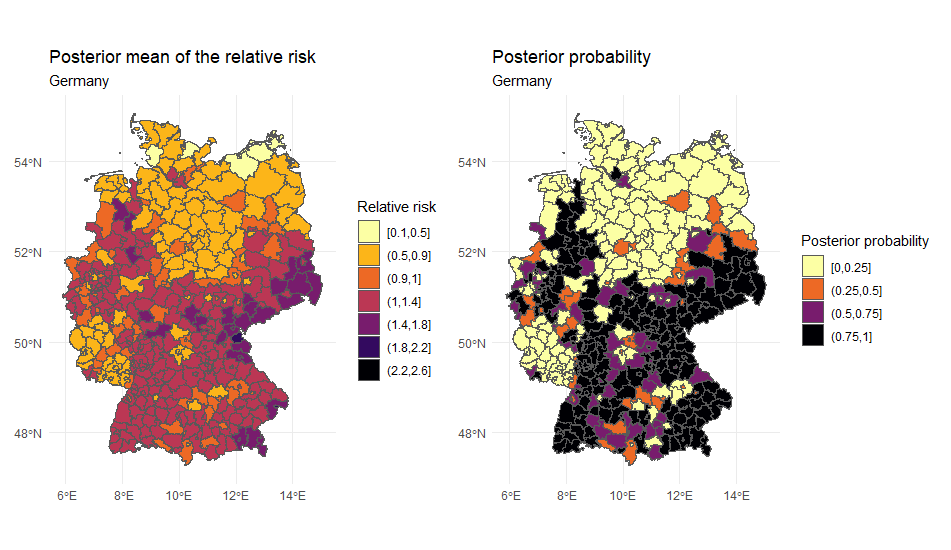
\includegraphics[width = \textwidth]{posterior_germany_demo.png}
    \caption{Posterior mean of the area-specific risk and the posterior probability.}
    \label{posteriorGermanyDemo}
\end{figure}
% \begin{figure}[H]
%     \centering
%     \includesvg[width = textwidth]{posterior_germany_demo.svg}
%    \caption{Posterior mean of the area-specific risk and the posterior probability.}
%     \label{posteriorGermanyDemo}
% \end{figure}
Compared to the standardised incidence rate in Germany, shown in Figure~\ref{sirgermany}, it can be seen that the parts of Germany with the lowest SIR, Northern Germany, are also the parts of Germany with the lowest relative risk. Saxony had the highest SIR and also has an increased relative risk. Most parts of Germany that had an SIR of around 1 have a relative risk between 1 and 1.4.
\paragraph{Infrastructure Models}$\newline$
Comparing Table~\ref{infraGermany_nospatial} and Table~\ref{infraGermany}, it can be seen that the model without spatial component performs slightly better in terms of the mean absolute error, equally well in terms of the CPO and worse in terms of the DIC and WAIC. \\
In the model without the spatial component, only population density and urban density had a significant effect, while in the BYM2 model, population density, number of retail shops and number of higher education buildings had a significant effect. \\
The posterior mean of the intercept implies a risk rate of -7.7\% for Germany with a credibility interval of -8.9\% to -6.4\%. \\
A 1 standard deviation increase in population density leads to a 9.4\% increase in relative risk, which is lower than the demographic model where it led to an 11.2\% increase. \\
The other significant effect associated with a higher risk of infection is the number of retail shops, as a 1 standard deviation increase in the number of retail shops leads to a 4.2\% increase in the risk of infection. A study by Barbieri et. al. analysed the content of Italian occupations working in about 600 sectors, with a focus on the dimensions that put workers at risk of infection during the Covid 19 pandemic. Their findings included that the retail sector appears to be at higher risk of infection
due to physical proximity in the workplace \autocite[][]{barbieri2020italian}. \\
The number of higher education buildings, i.e. colleges and universities, in a community reduces the risk of infection, as an increase of 1 standard deviation leads to a risk reduction of about 5.7\%. A possible explanation for this could be that in areas with more university buildings, the average education level of the population is higher. However, in a study by Plohl et. al. it was found that trust in science was positively correlated with compliance with COVID-19 prevention guidelines, but no relationship was found between trust in science and education level \autocite[][]{plohl2021modeling}.
\\
Figure~\ref{posteriorGermanyInfra} looks quite similar to Figure~\ref{posteriorGermanyDemo}, except for Saxony, where the relative risk is now above 2.2 for several municipalities, in addition to the one municipality that had such a risk level in Figure~\ref{posteriorGermanyDemo}. Furthermore, some other municipalities in Saxony and Thuringia also have higher relative risks compared to the demographic model.
\begin{figure}[H]
    \centering
    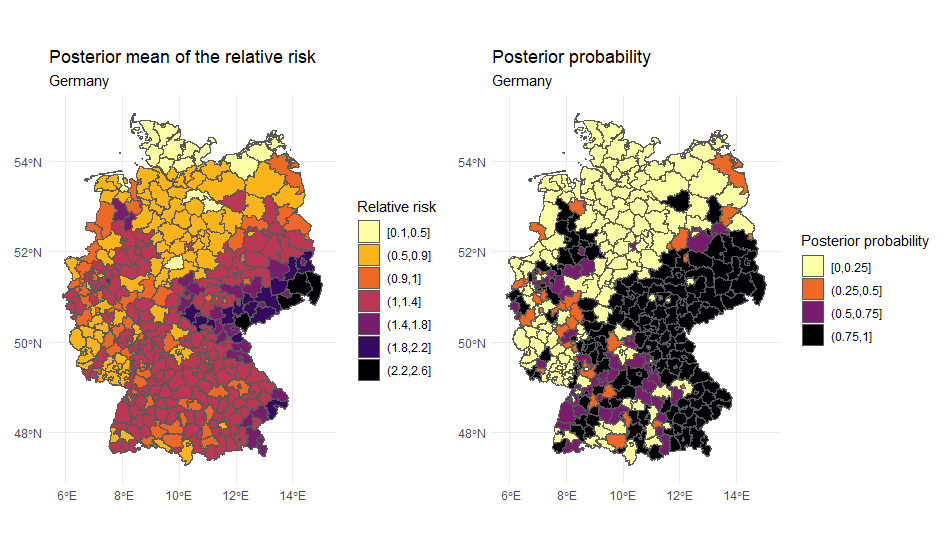
\includegraphics[width = \textwidth]{posterior_germany_infra.png}
    \caption{Posterior mean of the area-specific risk and the posterior probability.}
    \label{posteriorGermanyInfra}
\end{figure}
% \begin{figure}[H]
%     \centering
%     \includesvg[width = \textwidth]{posterior_germany_infra.svg}
%     \caption{Posterior mean of the area-specific risk and the posterior probability.}
%     \label{posteriorGermanyInfra}
% \end{figure}
\paragraph{Demographic + Infrastructure Models}$\newline$
Comparing Table~\ref{allGermany_nospatial} and Table~\ref{allGermany}, it can be seen that the model without spatial component performs equally well in terms of the CPO but worse in terms of the DIC, WAIC and MAE. \\
In the model without the spatial component, the significant effects include population density, the percentage of the vote for the FDP, the proportion of women, the logarithmic trade tax and the percentage of the vote for the SPD, die Linke and the Greens. For the BYM2 model, on the other hand, only population density and the percentage of the vote for the Greens are significant effects. \\
The posterior mean of the intercept implies a risk rate of -8.2\% for Germany with a credibility interval of -9.6\% to -6.7\%. \\
A 1 standard deviation increase in population density leads to a risk increase of 11.9\%, while a 1 standard deviation increase in the percentage of the vote for the Greens leads to a risk decrease of 14.5\%. What might cause these effects has already been discussed in section~\ref{par:demoGermany}. \\
When looking at Figure~\ref{posteriorGermanyAll}, it is difficult to distinguish it from Figure~\ref{posteriorGermanyDemo} because, except for a few municipalities, the posterior mean and posterior probability are mostly identical.
\begin{figure}[H]
    \centering
    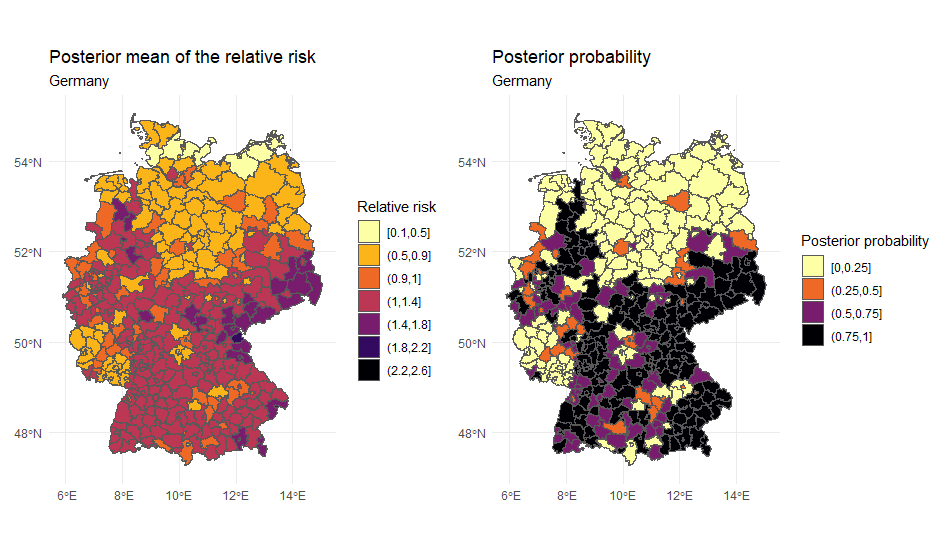
\includegraphics[width = \textwidth]{posterior_germany_all.png}
    \caption{Posterior mean of the area-specific risk and the posterior probability.}
    \label{posteriorGermanyAll}
\end{figure}
% \begin{figure}[H]
%     \centering
%     \includesvg[width = \textwidth]{posterior_germany_all.svg}
%     \caption{Posterior mean of the area-specific risk and the posterior probability.}
%     \label{posteriorGermanyAll}
% \end{figure}
\subsubsection{Discussion of the Models for Norway}
\paragraph{Demographic Models}$\newline$
Comparing Table~\ref{demoNorway_nospatial} and Table~\ref{demoNorway}, it can be seen that the model without spatial component performs better in terms of MAE, but worse in terms of DIC, WAIC and CPO. \\
In both models, only urban density has a significant impact on the risk of infection. \\
The posterior mean of the intercept implies a risk rate of -53.7\% for all of Norway. \\
A 1 standard deviation increase in urban density leads to a 7.9\% increase in the risk of infection. Since higher urban density means that there are more residential buildings in a given area, it should also be expected that there are more people in that area, which in turn facilitates the spread of a viral disease. \\
Looking at Figure~\ref{posteriorNorwayDemo}, excluding the two municipalities of Hyllestad and Ulvik, the risk is highest in the municipality of the nation's capital, Oslo, and the surrounding municipalities, with a posterior probability of at least 0.75 in all. In addition, a higher posterior mean can be observed in the western parts of southern Norway.
\begin{figure}[H]
    \centering
    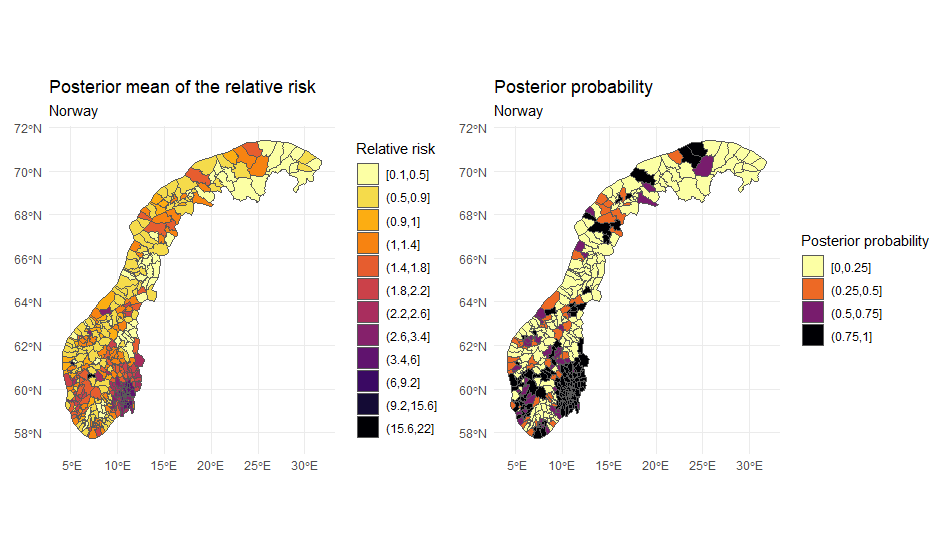
\includegraphics[width = \textwidth]{posterior_norway_demo.png}
    \caption{Posterior mean of the area-specific risk and the posterior probability.}
    \label{posteriorNorwayDemo}
\end{figure}
% \begin{figure}[H]
%     \centering
%     \includesvg[width = \textwidth]{posterior_norway_demo.svg}
%     \caption{Posterior mean of the area-specific risk and the posterior probability.}
%     \label{posteriorNorwayDemo}
% \end{figure}
For better interpretability, the logarithmic posterior mean is shown in Figure~\ref{posteriorNorwayDemoLog}.
\begin{figure}[H]
    \centering
    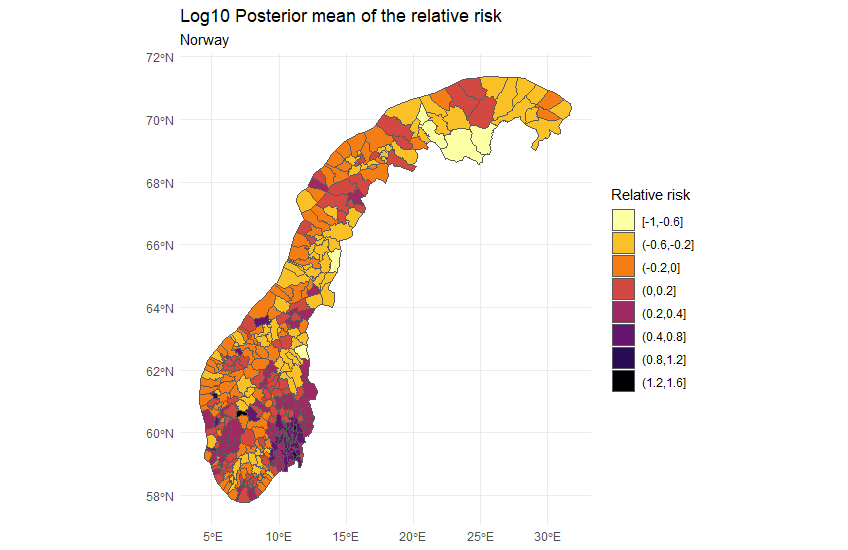
\includegraphics[width = \textwidth]{posterior_norway_demo_log.png}
    \caption{Logarithmic posterior mean of the area-specific risk.}
    \label{posteriorNorwayDemoLog}
\end{figure}
% \begin{figure}[H]
%     \centering
%     \includesvg[width = \textwidth]{posterior_norway_demo_log.svg}
%     \caption{Logarithmic posterior mean of the area-specific risk.}
%     \label{posteriorNorwayDemoLog}
% \end{figure}
Comparing the log relative risk with the log standardised incidence ratio in Figure~\ref{sirnorwaylog}, these two are quite similar. For most parts of Norway, the risk is at or below 0, while there is an increased risk in the Oslo region. However, there are a few municipalities that have a log-standardised incidence ratio of about 0, but a higher log-relative risk than this. Most of these are located in southern Norway, but a few are scattered throughout the rest of the country.
\paragraph{Infrastructure Models}$\newline$
Comparing Table~\ref{infraNorway_nospatial} and Table~\ref{infraNorway}, the BYM2 model outperforms the model without the spatial component in terms of every performance measure. \\
For the model without a spatial component, the urban density, the number of aerodromes in a municipality and the number of offices in a municipality has a significant effect on the risk of infection whereas in the BYM2 model only the number of places of worship significantly influences the risk of infection. \\
The intercept of the BYM2 model implies a risk rate of -67.2\% across Norway. \\
A 1 standard deviation increase in the number of places of worship in a given community leads to a 16.5\% increase in risk. Yezli and Khan, in a paper, advocate for the closure of places of worship and the suspension of religious gatherings because, in their opinion, these places pose a risk of transmission of Covid-19 to potentially large numbers of people through a single case. In addition, these gatherings often involve dense mixing of many people in a confined space, sometimes for extended periods of time \autocite[][]{yezli2020covid}. Wildman et. al. also examine the role of religion during the Covid 19 pandemic and conclude that religious community building directly influences virus spread by either inhibiting or accelerating social transmission, depending on which specific religious group is considered\autocite[][]{wildman2020religion}. \\
Looking at Figure~\ref{posteriorNorwayInfra} and Figure~\ref{posteriorNorwayInfraLog}, there is almost no difference to Figure~\ref{posteriorNorwayDemo} and Figure~\ref{posteriorNorwayDemoLog}.
\begin{figure}[H]
    \centering
    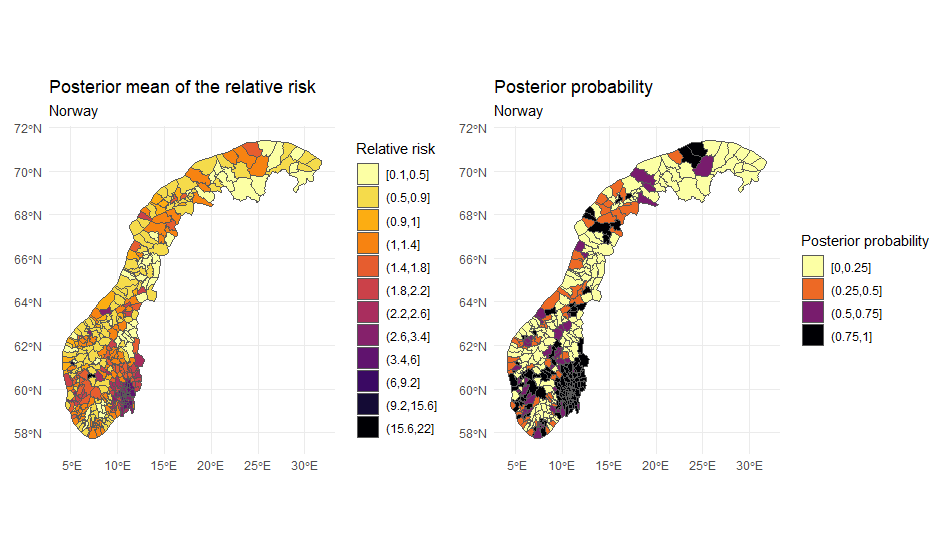
\includegraphics[width = \textwidth]{posterior_norway_infra.png}
    \caption{Posterior mean of the area-specific risk and the posterior probability.}
    \label{posteriorNorwayInfra}
\end{figure}
% \begin{figure}[H]
%     \centering
%     \includesvg[width = \textwidth]{posterior_norway_infra.svg}
%     \caption{Posterior mean of the area-specific risk and the posterior probability.}
%     \label{posteriorNorwayInfra}
% \end{figure}
\begin{figure}[H]
    \centering
    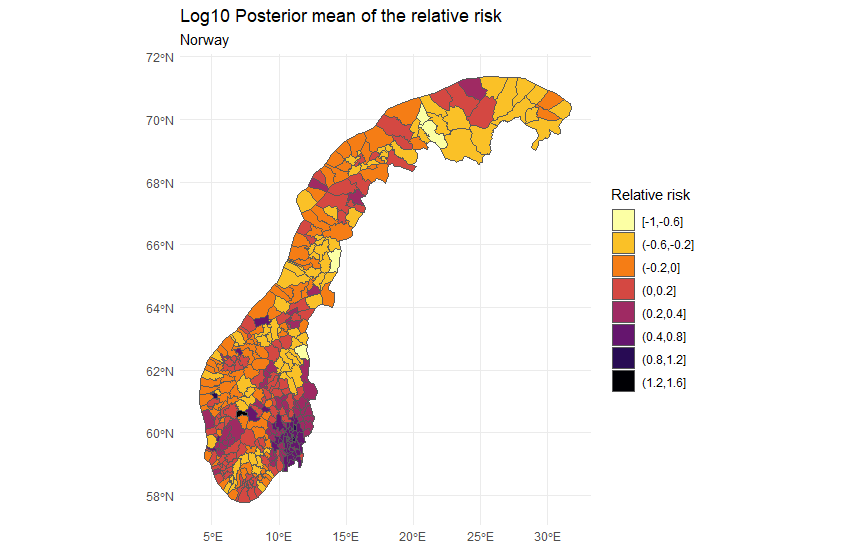
\includegraphics[width = \textwidth]{posterior_norway_infra_log.png}
    \caption{Logarithmic posterior mean of the area-specific risk.}
    \label{posteriorNorwayInfraLog}
\end{figure}
% \begin{figure}[H]
%     \centering
%     \includesvg[width = \textwidth]{posterior_norway_infra_log.svg}
%     \caption{Logarithmic posterior mean of the area-specific risk.}
%     \label{posteriorNorwayDemoLog}
% \end{figure}
\paragraph{Demographic + Infrastructure Models}$\newline$
Comparing Table~\ref{allNorway_nospatial} and Table~\ref{allNorway}, it can be seen that the model without spatial component performs better in terms of MAE, but worse in terms of DIC, WAIC and CPO. \\
For the model without the spatial component, the significant effects include the number of immigrants, the unemployment amongst immigrants, the urban density, the proportion of females and the number of aerodromes in a municipality. For the BYM2 model, there are only two significant effects, the number of immigrants as well as the median age in a municipality. \\
The intercept implies a -67.4\% risk rate across Norway. \\
A 1 standard deviation increase in the number of immigrants in a given community leads to a 15.6\% increase in risk. Finding the reason for this is difficult, some possible reasons could be barriers to adequate information due to low health literacy in certain groups and misconceptions about Covid-19 or testing criteria, as well as other socioeconomic and environmental factors, according to Indseth et. al. who published a paper in 2020 discussing the higher number of infections among immigrants in Norway \autocite[][]{indseth2020covid}.
In both models, only urban density has a significant impact on the risk of infection. \\
The posterior mean of the intercept implies a risk rate of -53.7\% for all of Norway. \\
A 1 standard deviation increase in urban density leads to a 7.9\% increase in the risk of infection. Since higher urban density means that there are more residential buildings in a given area, it should also be expected that there are more people in that area, which in turn facilitates the spread of a viral disease. \\
For the median age, an increase of 1 standard deviation leads to a risk reduction of 10.8\%, implying that people living in "younger" communities have a higher risk of infection. One possible reason for this could be that young people are more mobile and therefore come into contact with other people more often than older people. \\
When comparing Figure~\ref{posteriorNorwayAllLog} and Figure~\ref{posteriorNorwayInfraLog}, slight differences in the relative risk around the Oslo region can be seen. In Figure~\ref{posteriorNorwayAllLog}, the risk is higher northeast of Oslo and at the border to Sweden than in Figure~\ref{posteriorNorwayInfraLog}, while it is higher northwest of Oslo in Figure~\ref{posteriorNorwayInfraLog}, as well as in the northernmost regions of Norway.
\begin{figure}[H]
    \centering
    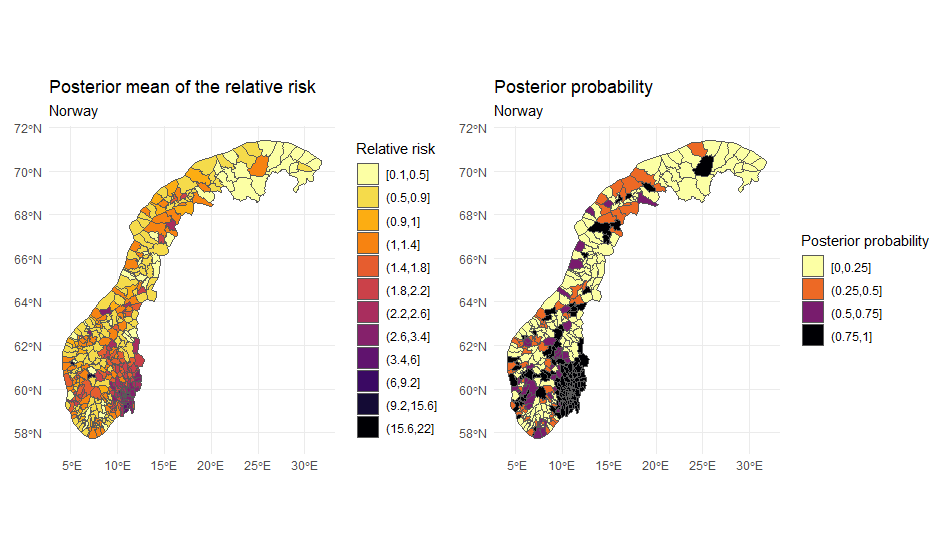
\includegraphics[width = \textwidth]{posterior_norway_all.png}
    \caption{Posterior mean of the area-specific risk and the posterior probability.}
    \label{posteriorNorwayAll}
\end{figure}
% \begin{figure}[H]
%     \centering
%     \includesvg[width = \textwidth]{posterior_norway_akk.svg}
%     \caption{Posterior mean of the area-specific risk and the posterior probability.}
%     \label{posteriorNorwayAll}
% \end{figure}
\begin{figure}[H]
    \centering
    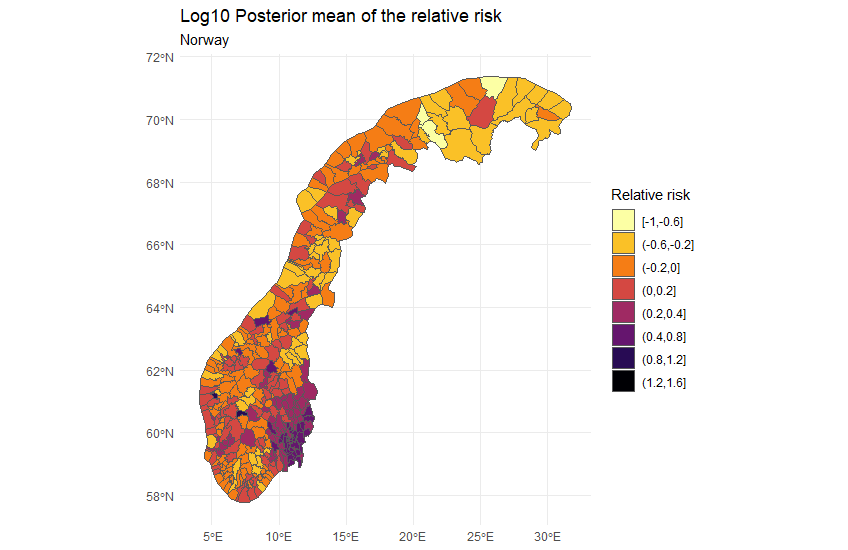
\includegraphics[width = \textwidth]{posterior_norway_all_log.png}
    \caption{Logarithmic posterior mean of the area-specific risk.}
    \label{posteriorNorwayAllLog}
\end{figure}
% \begin{figure}[H]
%     \centering
%     \includesvg[width = \textwidth]{posterior_norway_all_log.svg}
%     \caption{Logarithmic posterior mean of the area-specific risk.}
%     \label{posteriorNorwayAllLog}
% \end{figure}
\subsection{Choice of Prior Sensitivity}
As can be seen in equation~\ref{pcprec}, there is flexibility when it comes to choosing the values for the standard deviation $\sigma_0$ as well as the probability $\alpha$. Therefore, an upper bound for the standard deviation can be chosen as well as the weight placed on this "tail event", describing how informative the resulting prior is. In the following, an assessment is made of how the performance of a Besag model, a BYM2 model and a Leroux model changes when playing around with the value for the standard deviation $\sigma_0$. \\
By allowing the precision to be greater, the variance is forced to be smaller. Hence, choosing a higher value for the precision leads to lower values for the DIC, WAIC and CPO, as can be seen in Figure~\ref{comparison_norway_1} and Figure~\ref{comparison_norway_2}. While this indicates a better fit to the training data, Figure~\ref{comparison_norway_2} also shows that the MAE increases when a higher value for $U=\sigma_0$ is chosen, as the models overfit on the training data and therefore make worse predictions. \\
The corresponding figures for Germany are shown in Figure~\ref{comparison_germany_1} and Figure~\ref{comparison_germany_2} in the Appendix.
\begin{figure}[H]
    \centering
    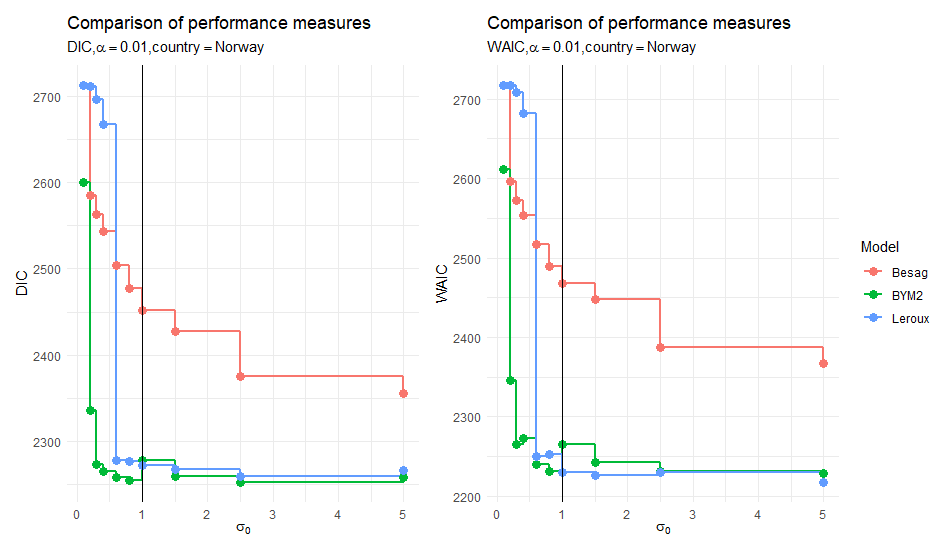
\includegraphics[width = \textwidth]{comparison_1_norway.png}
    \caption{Value of the DIC and WAIC when changing the value for $\sigma_0$. The black line highlights the values for $\sigma_0$ = 1.}
    \label{comparison_norway_1}
\end{figure}
% \begin{figure}[H]
%     \centering
%     \includesvg[width = \textwidth]{comparison_1_norway.svg}
%     \caption{Value of the DIC and WAIC when changing the value for $\sigma_0$. The black line highlights the values for $\sigma_0$ = 1.}
%     \label{comparison_norway_1}
% \end{figure}
\begin{figure}[H]
    \centering
    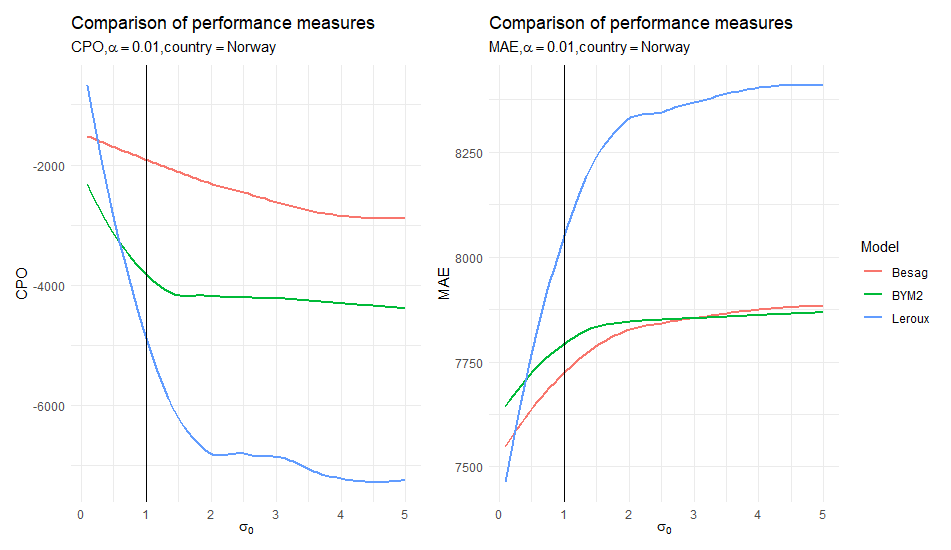
\includegraphics[width = \textwidth]{comparison_2_norway.png}
    \caption{Value of the CPO and MAE when changing the value for $\sigma_0$. The black line highlights the values for $\sigma_0$ = 1.}
    \label{comparison_norway_2}
\end{figure}
% \begin{figure}[H]
%     \centering
%     \includesvg[width = \textwidth]{comparison_2_norway.svg}
%     \caption{Value of the CPO and MAE when changing the value for $\sigma_0$. The black line highlights the values for $\sigma_0$ = 1.}
%     \label{comparison_norway_2}
% \end{figure}
\section{Spatio-Temporal Models}
\subsection{Spatio-Temporal Models for Germany}
\subsection{Spatio-Temporal Models for Norway}
\subsection{Discussion of the Spatio-Temporal Models}
\clearpage
\section{Predictive Models}
\subsection{Predictive Models for Germany}
\subsection{Predictive Models for Norway}
\subsection{Discussion of the Predictive Models}
% TODO: Variance Inflation Score
% TODO: How to calculate posterior mean of the relative risk
% TODO: How to calculate posterior probability
% TODO: Diese Transformation da
% As this was the overall best-performing spatial model for Germany, a look is taken at the posterior means $\pmb{\zeta} = \exp{\left(\xi\right)}$ of the area-specific risks. Since the uncertainty associated with them can also be mapped, the posterior probability $\mathbb{P}\left(\zeta_i > 1|\pmb{y}\right)$ is visualised as well.